\documentclass[12pt]{dalthesis}
\usepackage{amsmath,graphicx}

\begin{document}

\title{Adiabatic Quantum Computation}
\author{Elliot Snow-Kropla}
%\date{20 July 2012}

\degree{Master of Science}
\degreeinitial{M.Sc.}
\faculty{Faculty of Science}
\dept{Department of Physics and Atmospheric Science}

\defencemonth{August}\defenceyear{2014}

\frontmatter

\begin{abstract}
	Lorum Ipsum
\end{abstract}

\begin{acknowledgements}
	Nobody! Hahaha
\end{acknowledgements}

\mainmatter

\chapter{Introduction}

\chapter{Adiabatic Quantum Computing}
Introduced by Farhi et.\ al.\cite{farhi}, the idea of adiabatic quantum computation (hereafter AQC) is to exploit the adiabatic theorem to solve computational problems.  There are two main components to the idea.  First, we find a Hamiltonian such that the ground state is the solution to a computational problem (e.g. a bitstring of spins pointed up and down).  Second, we use the adiabatic theorem to move from some easily prepared initial state into the Hamiltonian we found.

\section{Finding a Problem Hamiltonian}
While in principle there are an unlimited number of ways to construct a Hamiltonian whose ground state encodes the solution to a computation, our method is to use an N-particle Hamiltonian of the form

\begin{displaymath}
	H = \sum_{i} h_i \sigma_i^Z + \sum_{i < j} J_{ij} \sigma_i^Z\sigma_j^Z
\end{displaymath}

where $\sigma_i^Z$ is the pauli matrix of the ith particle and $h_i$ and $J_{ij}$ are the parameters of the Hamiltonian.  This 2-local Hamiltonian corresponds to a graph structure, where each particle is a vertex and each non-zero $J_{ij}$ is an edge, while non-zero $h_i$s can be represented as edges to a constant "field" spin.

Our problem of finding a suitable Hamiltonian is now reduced to finding a set of $h$'s and $J_{ij}$'s such that our desired solution is encoded in the ground state.

\section{Adiabatic Evolution}

\chapter{Embedding}
Because in general programs compiled to Ising graphs can be of any shape, we need a way to convert arbitrary graphs into Chimera graphs that can be executed on a machine.  This is done by adding \emph{clone spins} into the graph: each clone spin has the same value in the ground state as one of the logical spins in the input graph.  Thus we can decrease the connectivity of the input graph until it is sparse enough to be isomorphic to a physical machine.

\section{ Embedding algorithm}

The embedding algorithm is as follows:

\emph{\textbf{Definitions:}}

Designate the input Hamiltonian graph $V$ and the output Chimera graph $G$.  Label the spins in $V$ and $G$ as $V_i$ and $G_i$ respectively.
We define the \emph{clone map} $C_i$ as the set of spins $[i,j \ldots]$ which have the same logical value as their parent spin: so for example the clone map of spin 5, $C_5$, might be $[2,3,13]$ which would mean that spins 2, 3, 5 and 13 all share the same logical value.  We define a mapping $M$ between logical spins in graph $V$ and computation spins in graph $G$.  

We also define a \emph{clone coupling} value which is as large as possible and ferromagnetic; this attempts to ensure that all the members of a clone map are aligned in the ground state.  In the final $G$, each member of a clone map should have a clone coupling connecting it to at least one other member of the clone map.

\emph{\textbf{Procedure:}}
\begin{enumerate}
	\item Populate $M$ by mapping each $V_i$ to one of the spins $G_j$ on the left side of a qubyte that lies along the diagonal of $G$
	\item For each field term in $V$, add a field to $G$ on the corresponding spin
	\item For each $J_{ij}$ in $V$, conduct the following operation:
		\begin{itemize}
			\item Scan through both of $C_i$ and $C_j$ to find the pair which are nearest to each other in $G$; call these $x$ and $y$
			\item Get a list of each spin that lies along the path between $x$ and $y$
			\item Assign half of these spins to $C_i$ and half to $C_j$; add the appropriate clone coupling into $G$ for each spin in the path to ensure that the clone map is properly connected
			\item Finally, at the interface between the two new clone map members, add a coupling into $G$ with the same value as $J_{ij}$
		\end{itemize}
\end{enumerate}

Each term in $V$, both fields and couplings, should now have a corresponding term in $G$.  $G$ should also contain many coupling terms that group the necessary clone maps.

\chapter{Preliminary Results}

\begin{figure}
	\scalebox{0.3}{
	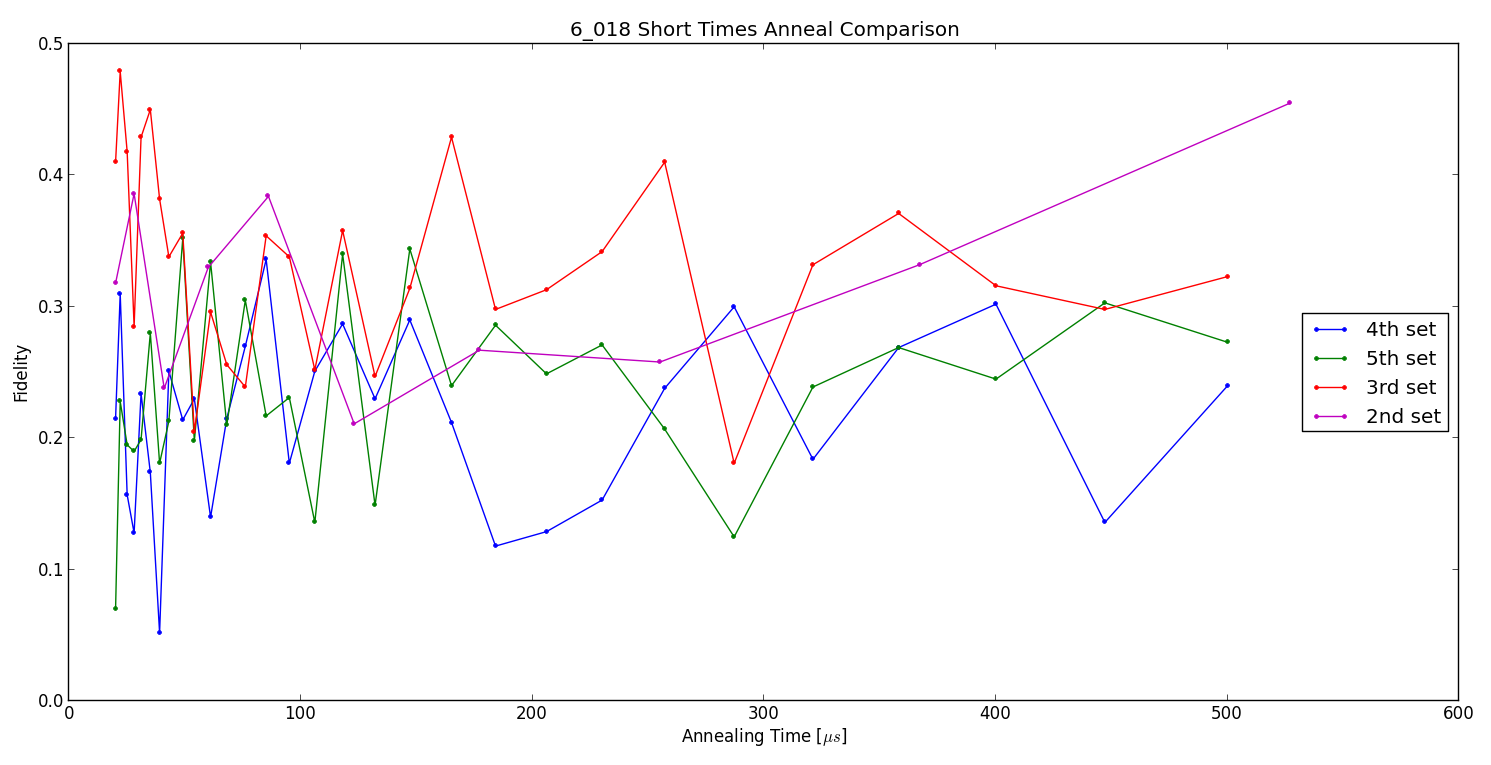
\includegraphics[bb=0 0 745 382]{img/6_018_comparison.png}
}
	\caption[Fidelity vs Time]{Plot of the fidelity as a function of annealing time for the Hamiltonian ``k44'' from several different machine runs.}
	\label{fid_v_time}
\end{figure}

Figure \ref{fid_v_time} shows the results of 50,000 runs of the annealing machine consisting of 1000 runs at various annealing times.  Along the y-axis is the fidelity, and along the x-axis is the annealing time.  Contrary to what we expect from the adiabatic theorem and simulations of quantum annealing the fidelity is uncorrelated with annealing from 20$\mu$s out to roughly 500$ \mu$s, after which the fidelity \emph{decreases} with increasing annealing time.  This unexpected behaviour leaves us with a number of questions:

\begin{itemize}
	\item For long annealing times, why does the fidelity decrease with increasing annealing times?
	\item For short annealing times, why does the fidelity appear insensitive to annealing time?
	\item Is the short time fidelity dominated by the Hamiltonian programming noise?
	\item Is there significant drift in the fidelities after programming?
	\item Does the Hamiltonian fidelity depend strongly on the number of coupling values?
\end{itemize}

\bibliographystyle{plain}
\bibliography{eskthesis}
\end{document}
